\documentclass[tikz,border=2pt]{standalone}
\usepackage{graphicx}
\usepackage{xcolor}
\usepackage[scaled=0.93]{helvet}
\renewcommand{\familydefault}{\sfdefault}

\definecolor{UTBurnt}{RGB}{191,87,0}
\definecolor{UTDark}{RGB}{51,63,72}
\definecolor{UTLight}{RGB}{248,246,242}

\begin{document}
\begin{tikzpicture}
  \node[anchor=north west,inner sep=0pt] (testbed) at (0,0)
    {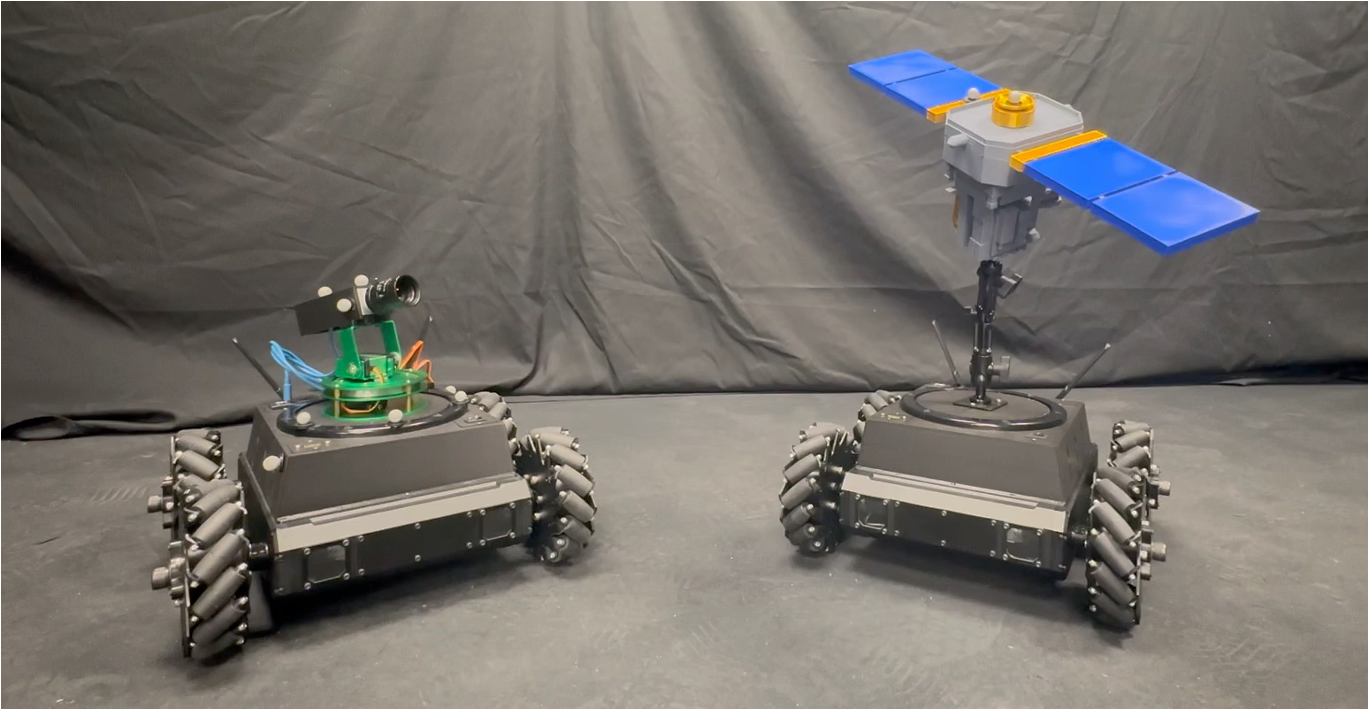
\includegraphics[width=12.8cm]{fig_testbed_overview.png}};
  \node[anchor=north west,fill=UTBurnt,text=white,font=\bfseries\scriptsize,
        inner xsep=5pt,inner ysep=2pt] at (0.12,-0.12)
    {Robotic HIL Testbed};

  \node[anchor=north west,inner sep=0pt] (hardware) at (0,-6.65)
    {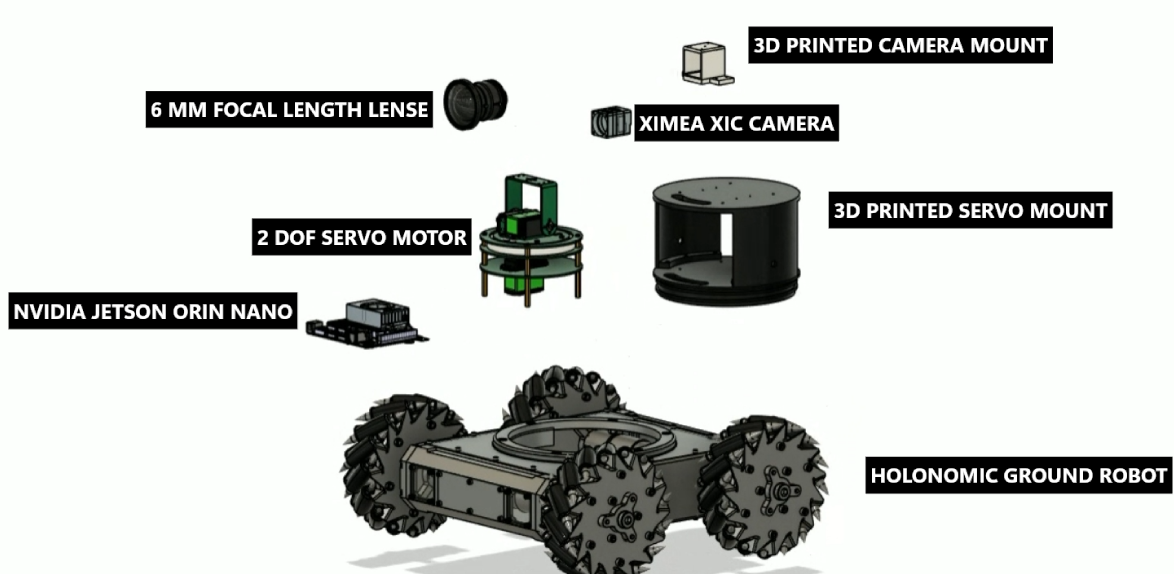
\includegraphics[width=12.8cm]{fig_hardware_exploded_view.png}};
  \node[anchor=north west,fill=UTBurnt,text=white,font=\bfseries\scriptsize,
        inner xsep=5pt,inner ysep=2pt] at (0.12,-6.77)
    {Onboard Sensing and Compute Stack};

\end{tikzpicture}
\end{document}
